\newpage
\chapter{Netsimile}

\section{Eindimensionales Signal urspr�ngliche Version}
\label{sec:appendix_net_original}
\begin{figure}
	\centering
	\subfloat[Ausrei�ertyp Signal Drift]{
		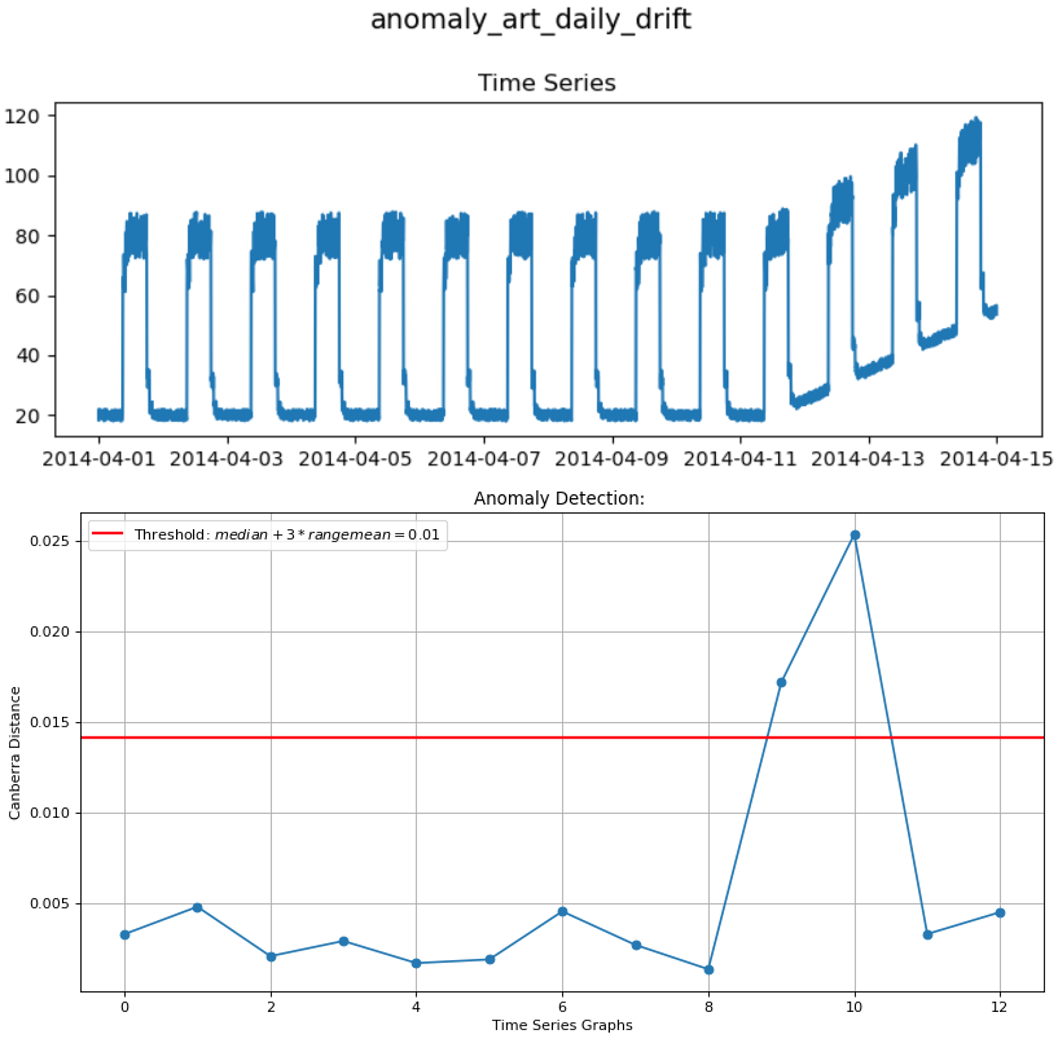
\includegraphics[width=0.5\textwidth]{fig/resultsNetismile/original/daily_drift}}
	\subfloat[Ausrei�ertyp Zunahme am Rauschen]{
		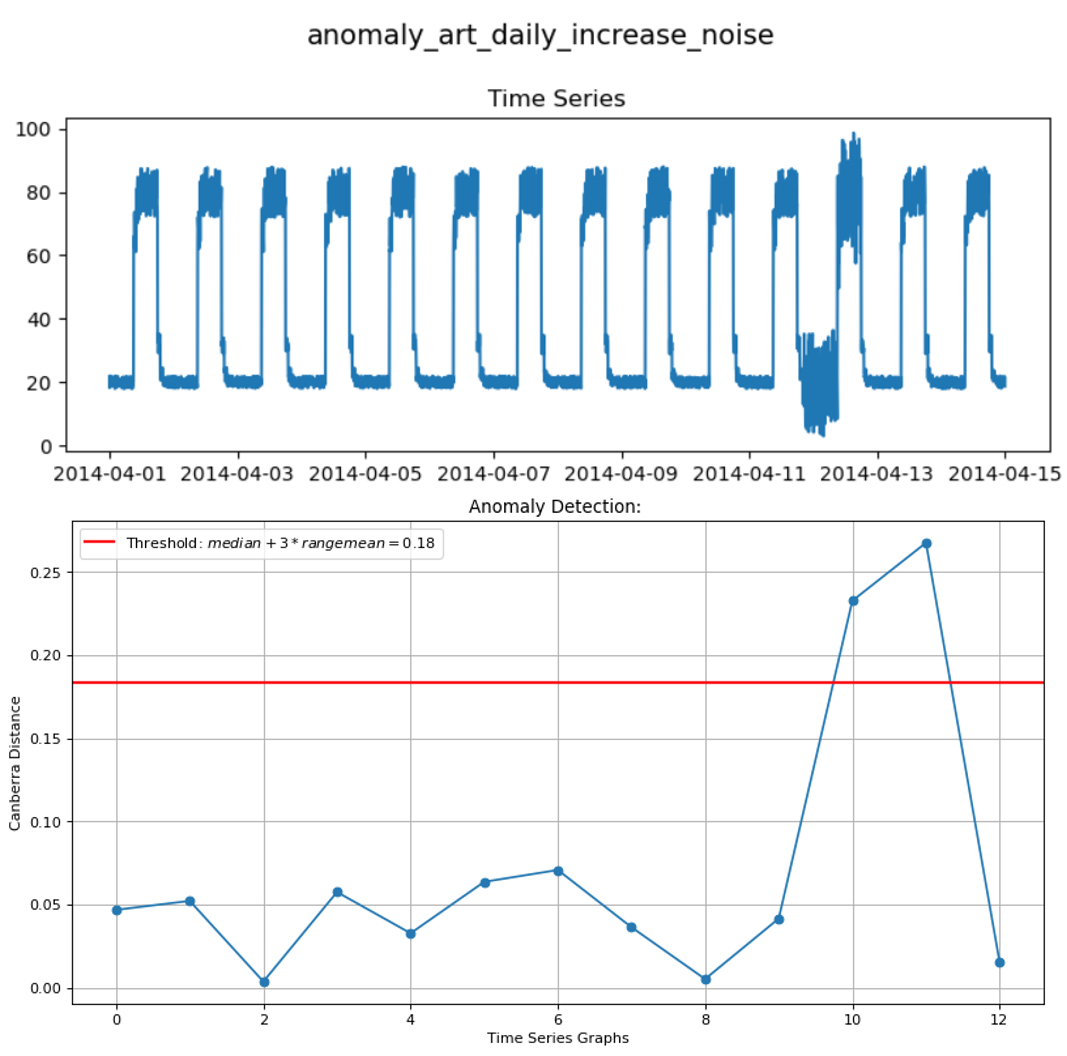
\includegraphics[width=0.5\textwidth]{fig/resultsNetismile/original/increase_noise}}
	\qquad
	\subfloat[Ausrei�ertyp Einzelne Peaks]{
		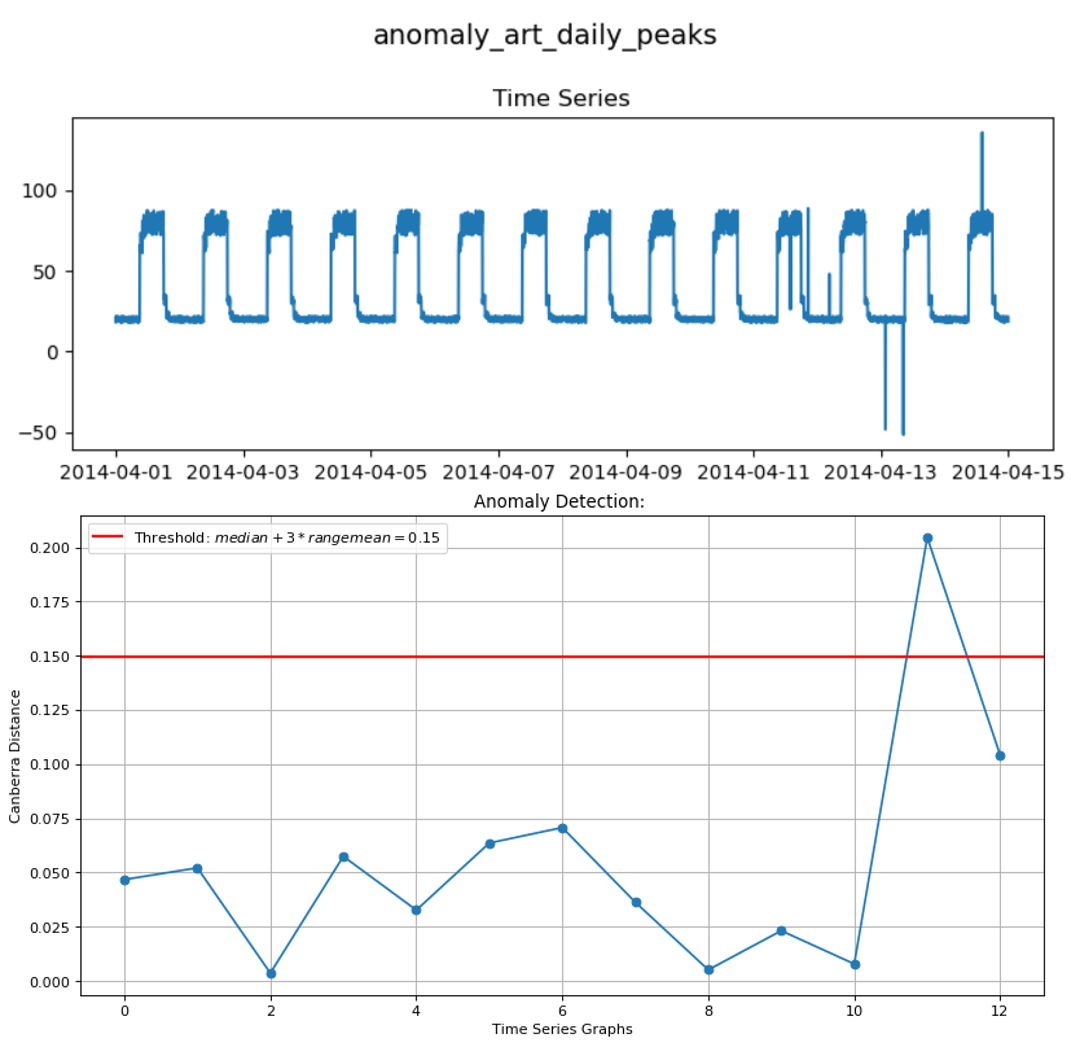
\includegraphics[width=0.5\textwidth]{fig/resultsNetismile/original/daily_peaks}}
	\subfloat[Ausrei�ertyp Frequenz�nderung]{		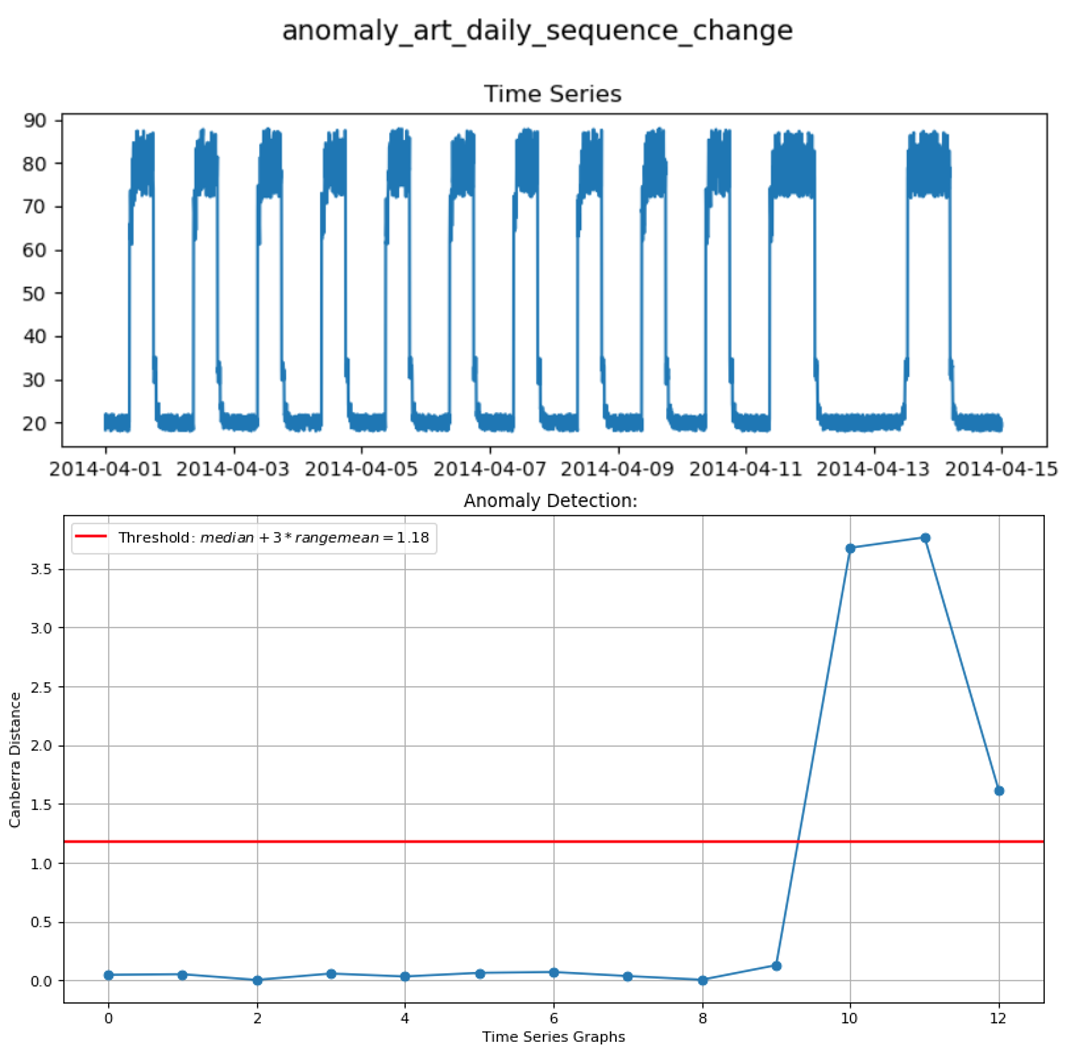
\includegraphics[width=0.5\textwidth]{fig/resultsNetismile/original/sequence_change}}
	\qquad
	\label{img:isomappictures1}
\end{figure}
\begin{figure}\ContinuedFloat
	\subfloat[Ausrei�ertyp Kontinuierliche Zunahme der Amplitude]{
		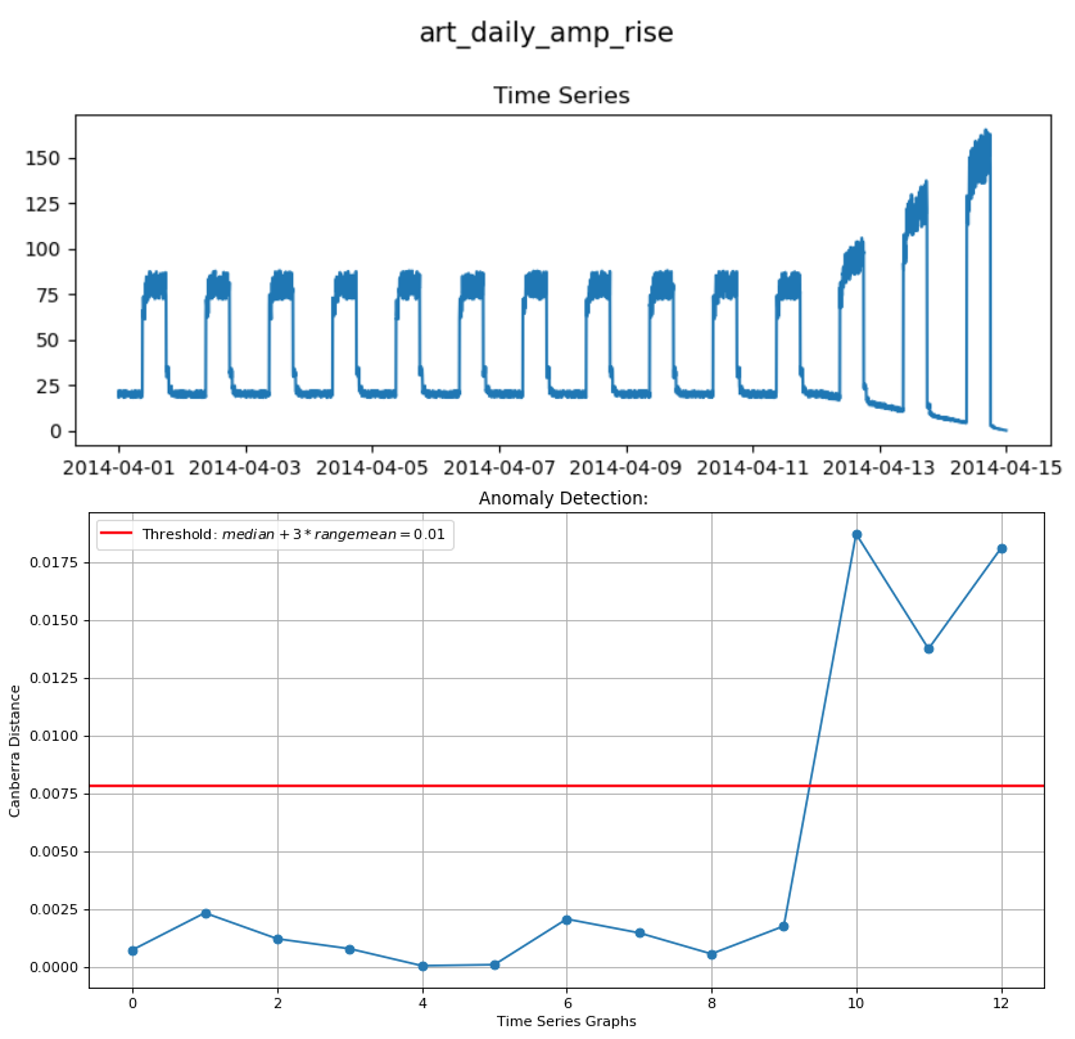
\includegraphics[width=0.5\textwidth]{fig/resultsNetismile/original/amp_rise}}
	\subfloat[Ausrei�ertyp Zyklus Aussetzer]{
		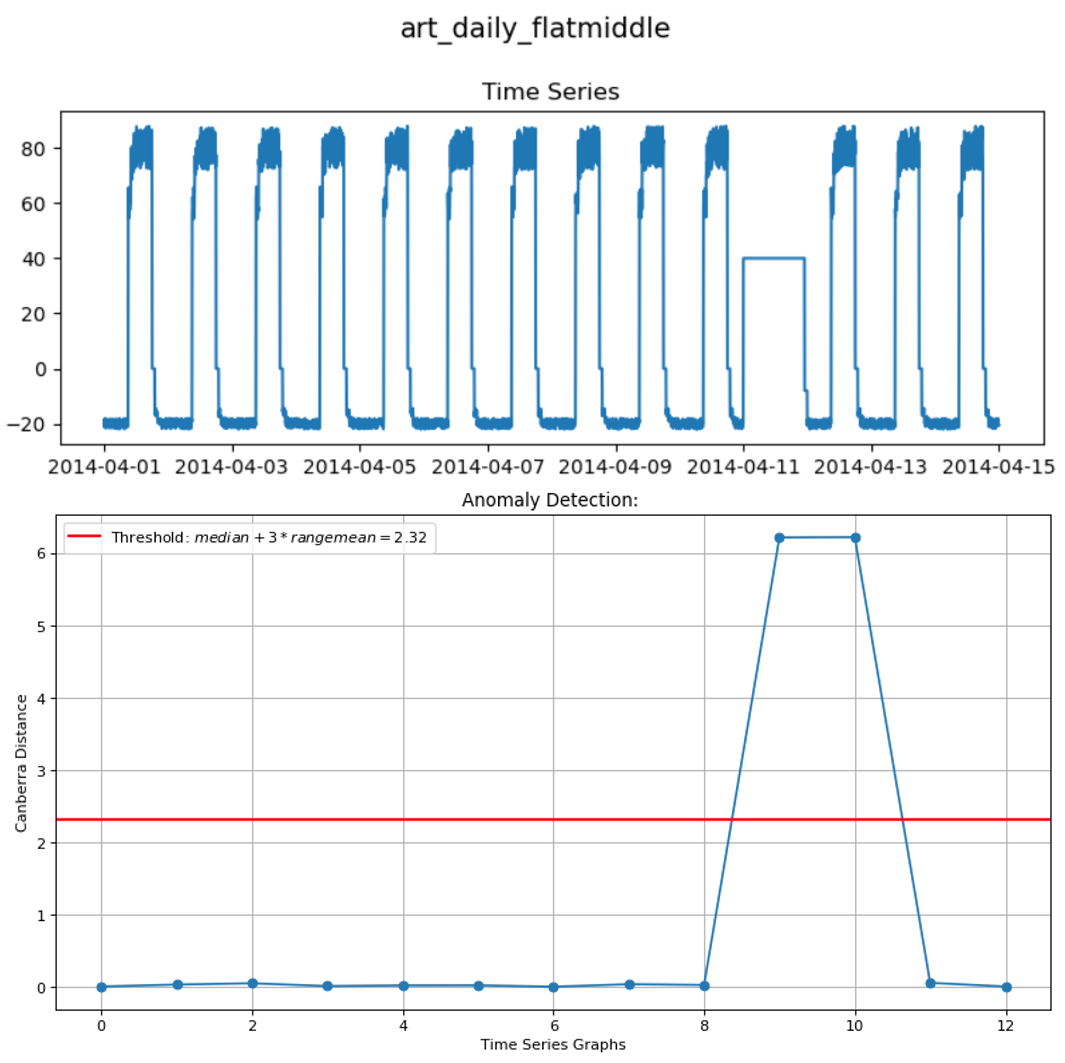
\includegraphics[width=0.5\textwidth]{fig/resultsNetismile/original/flatmiddle}}
	\qquad
	\subfloat[Ausrei�ertyp Zyklus mit geringerer Amplitude]{
		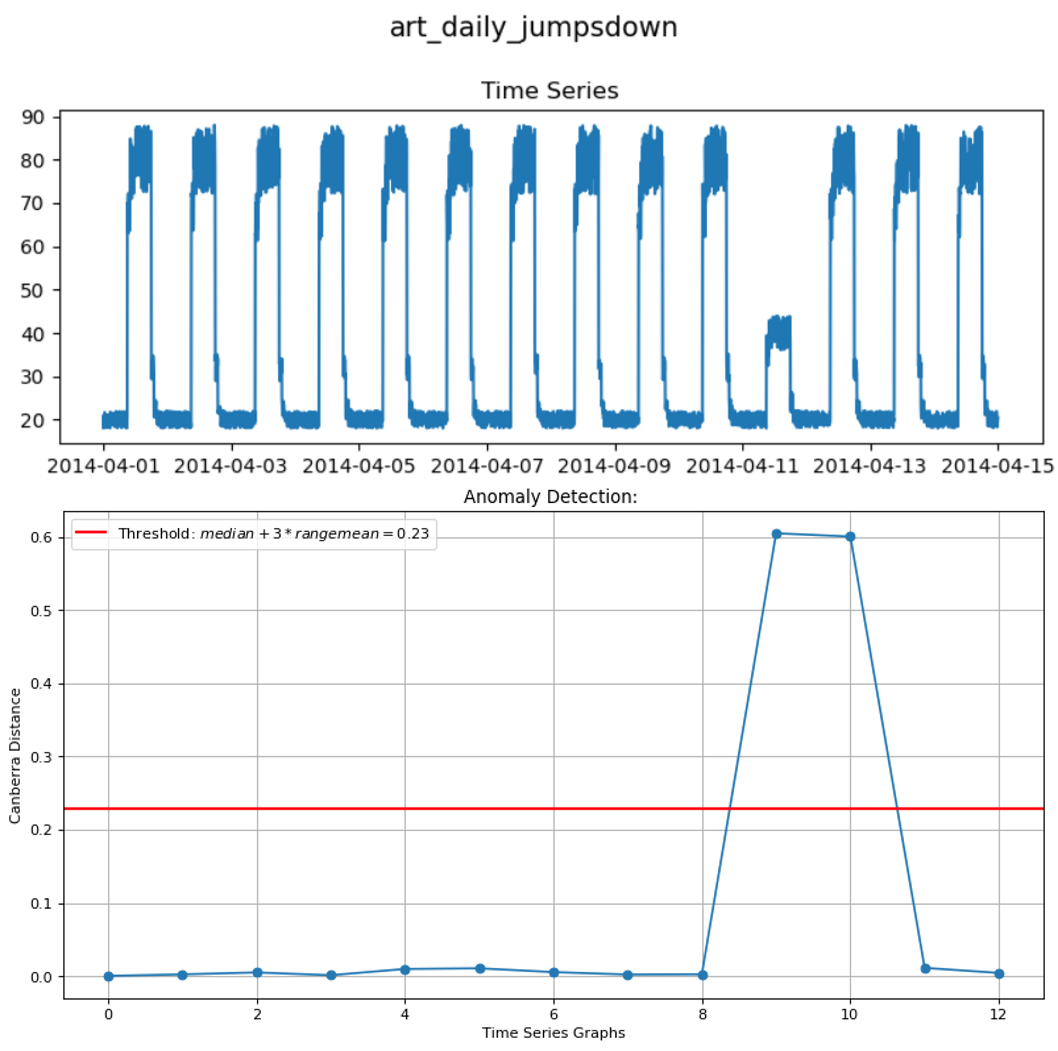
\includegraphics[width=0.5\textwidth]{fig/resultsNetismile/original/jumpsdown}}
	\subfloat[Ausrei�ertyp Zyklus mit h�herer Amplitude]{
		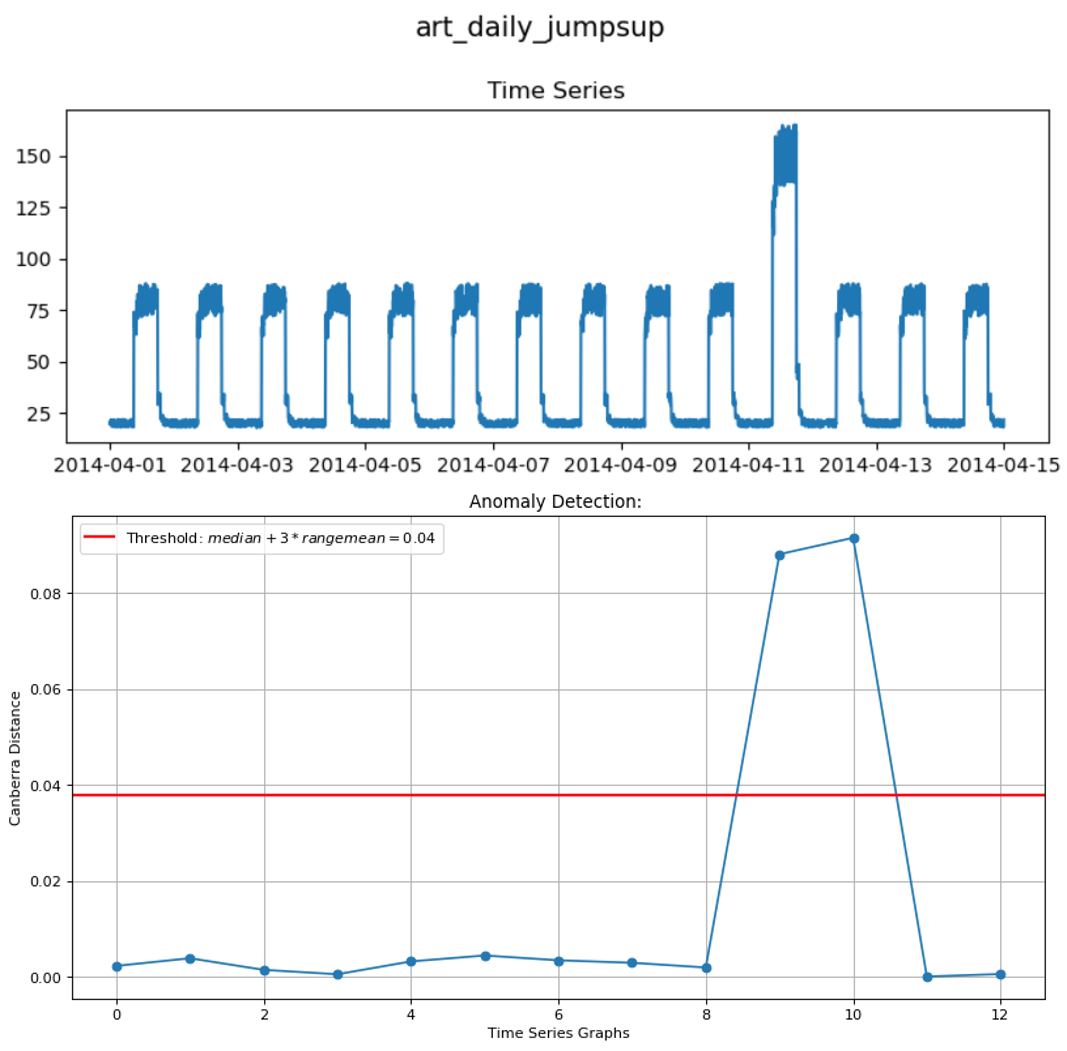
\includegraphics[width=0.5\textwidth]{fig/resultsNetismile/original/jumpsup}}
	\qquad
	\subfloat[Ausrei�ertyp Signal-Aussetzer]{
		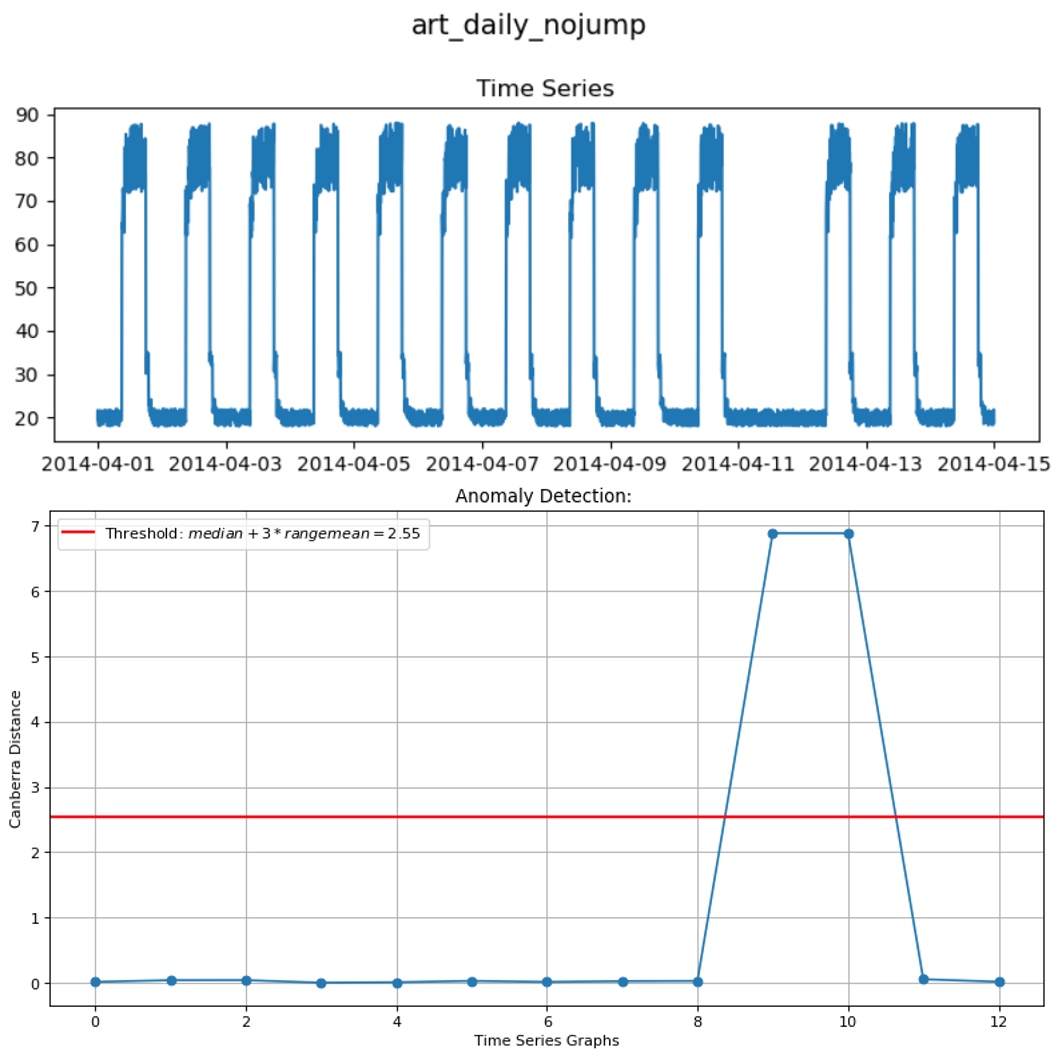
\includegraphics[width=0.5\textwidth]{fig/resultsNetismile/original/nojump}}
	\label{img:isomappictures2}
\end{figure}

\section{Eindimensionales Signal Optimierte Version}
\label{sec:appendix_net_one}
\begin{figure}
	\centering
	\subfloat[Caption for sub-figure1]{
		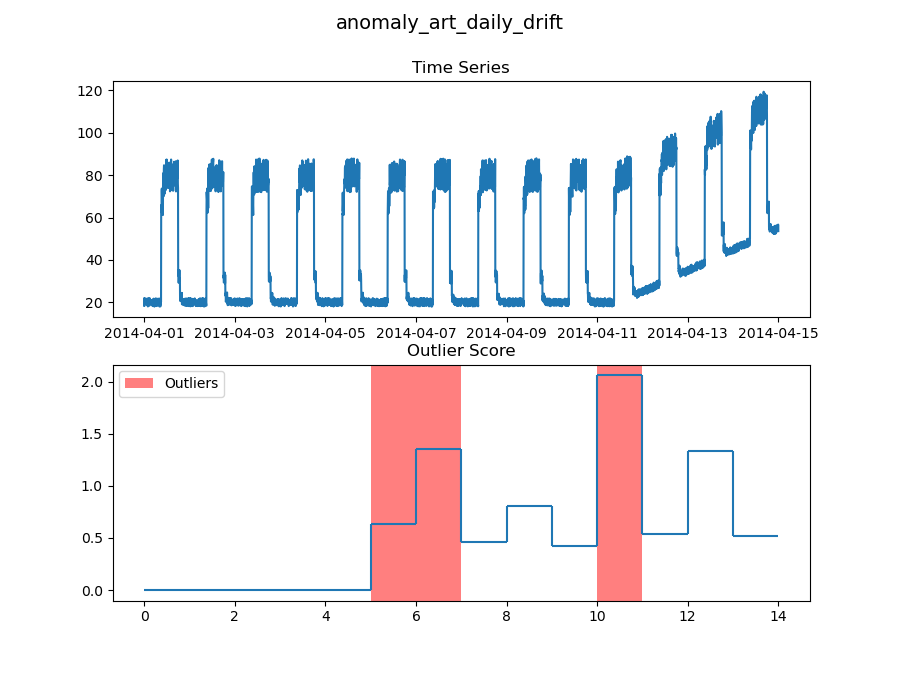
\includegraphics[width=0.5\textwidth]{fig/resultsNetismile/1D/anomaly_art_daily_drift}}
	\subfloat[Caption for sub-figure1]{
		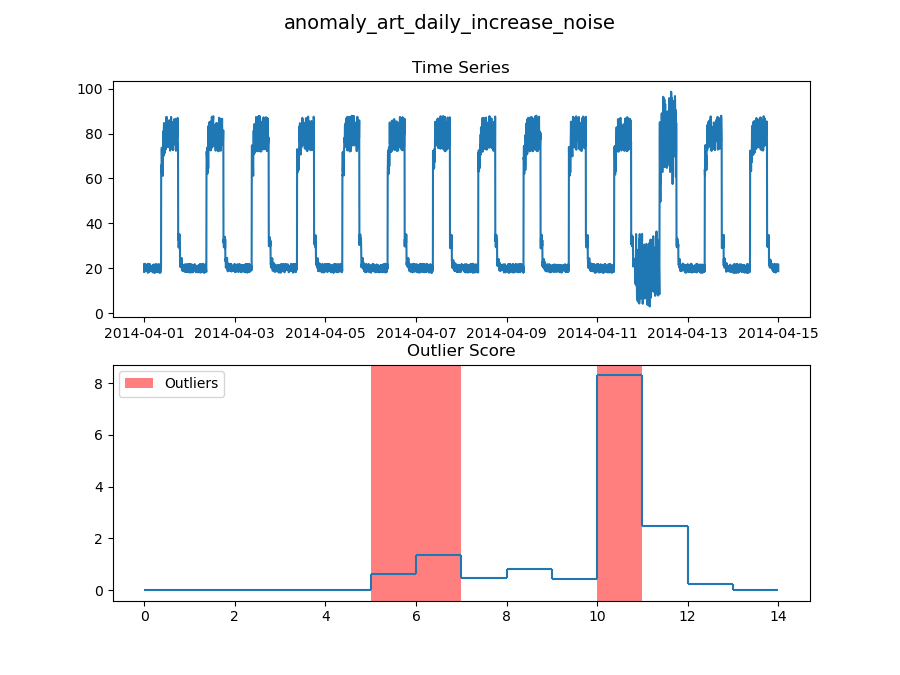
\includegraphics[width=0.5\textwidth]{fig/resultsNetismile/1D/anomaly_art_daily_increase_noise}}
	\qquad
	\subfloat[Caption for sub-figure1]{
		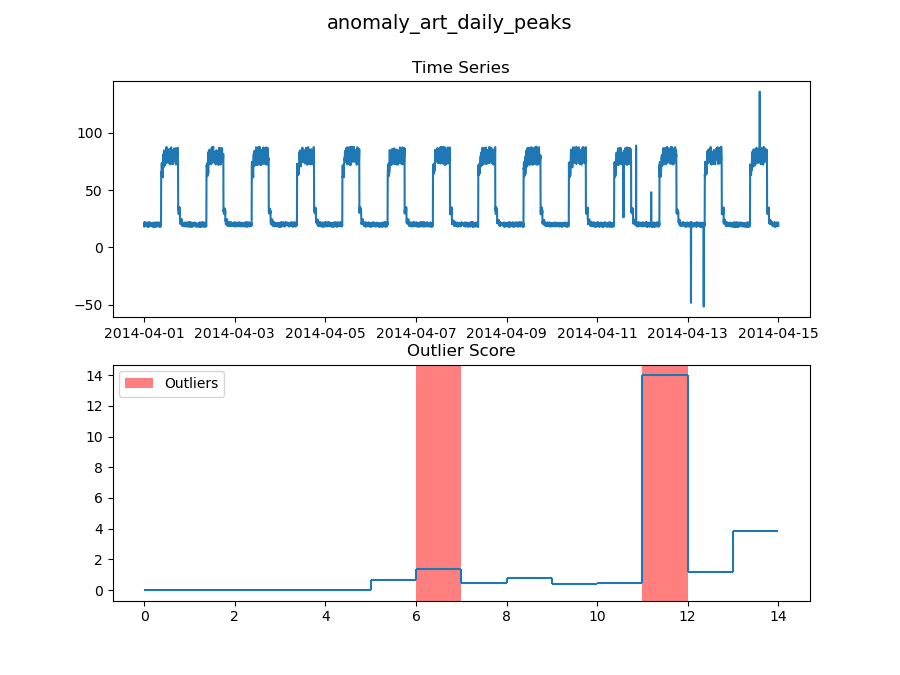
\includegraphics[width=0.5\textwidth]{fig/resultsNetismile/1D/anomaly_art_daily_peaks}}
	\subfloat[Caption for sub-figure1]{
		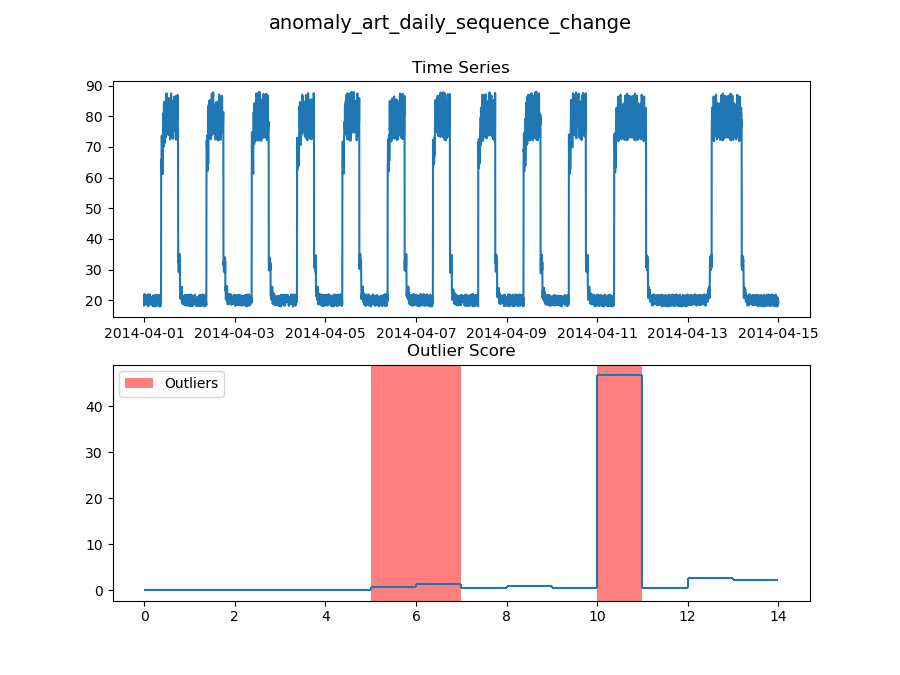
\includegraphics[width=0.5\textwidth]{fig/resultsNetismile/1D/anomaly_art_daily_sequece_change}}
	\qquad
	\label{img:isomappictures1}
\end{figure}
\begin{figure}\ContinuedFloat
	\subfloat[Caption for sub-figure1]{
		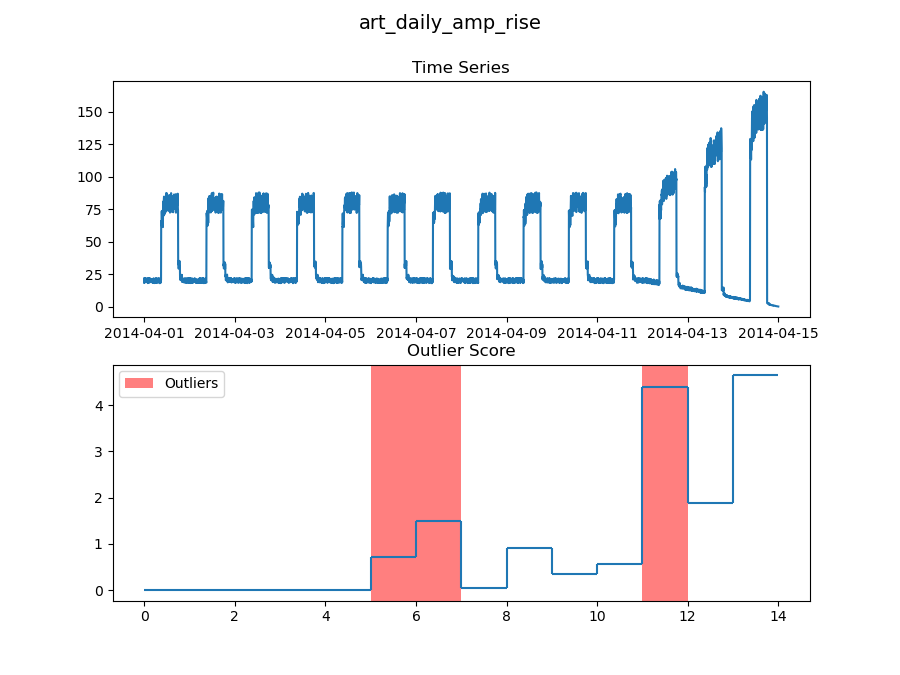
\includegraphics[width=0.5\textwidth]{fig/resultsNetismile/1D/art_daily_amp_rise}}
	\subfloat[Caption for sub-figure1]{
		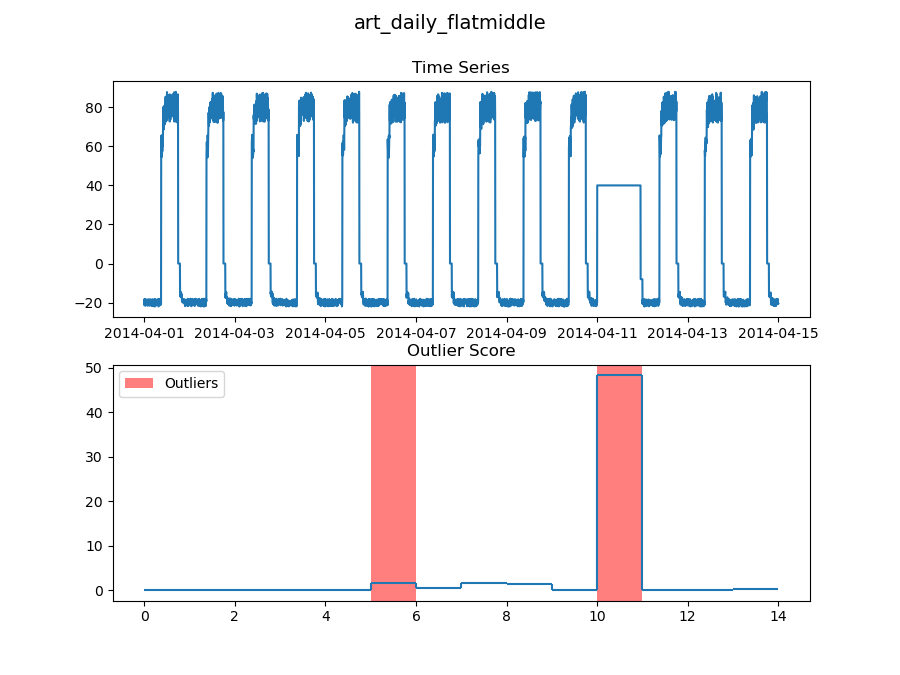
\includegraphics[width=0.5\textwidth]{fig/resultsNetismile/1D/art_daily_flatmiddle}}
	\qquad
	\subfloat[Caption for sub-figure1]{
		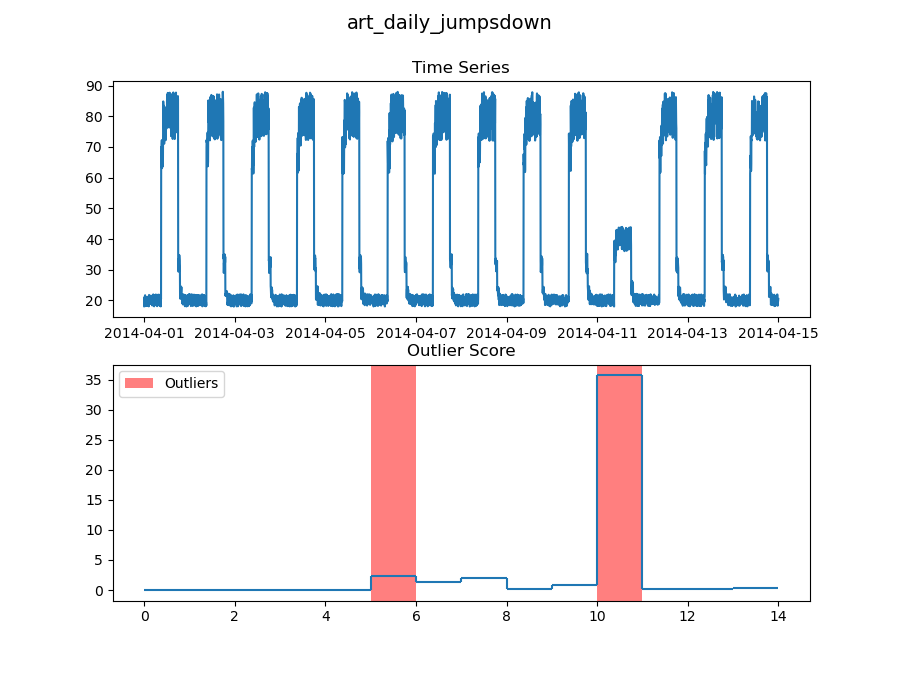
\includegraphics[width=0.5\textwidth]{fig/resultsNetismile/1D/art_daily_jumpsdown}}
	\subfloat[Caption for sub-figure1]{
		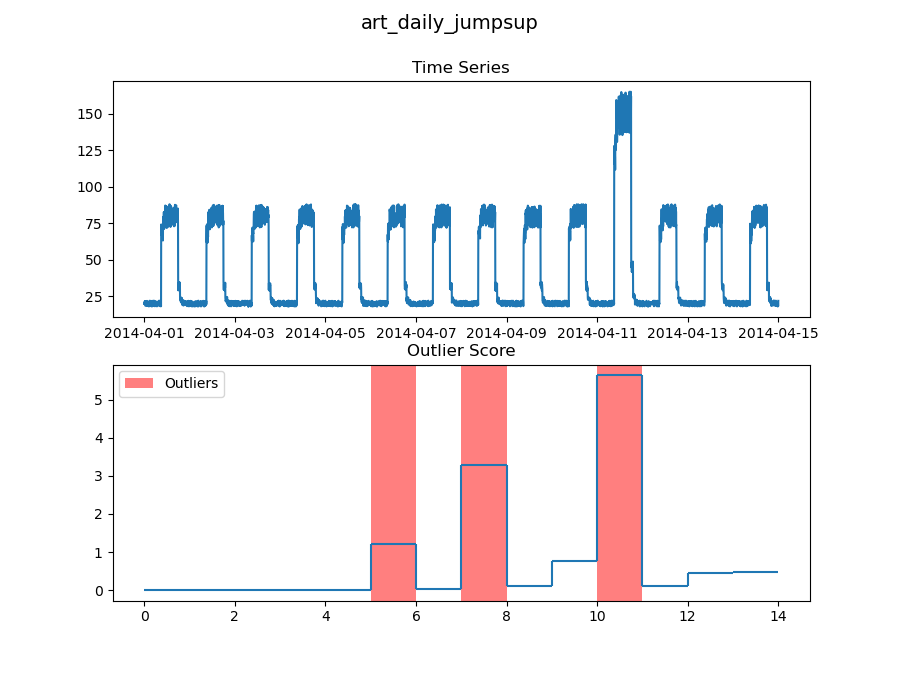
\includegraphics[width=0.5\textwidth]{fig/resultsNetismile/1D/art_daily_jumpsup}}
	\qquad
	\subfloat[Caption for sub-figure1]{
		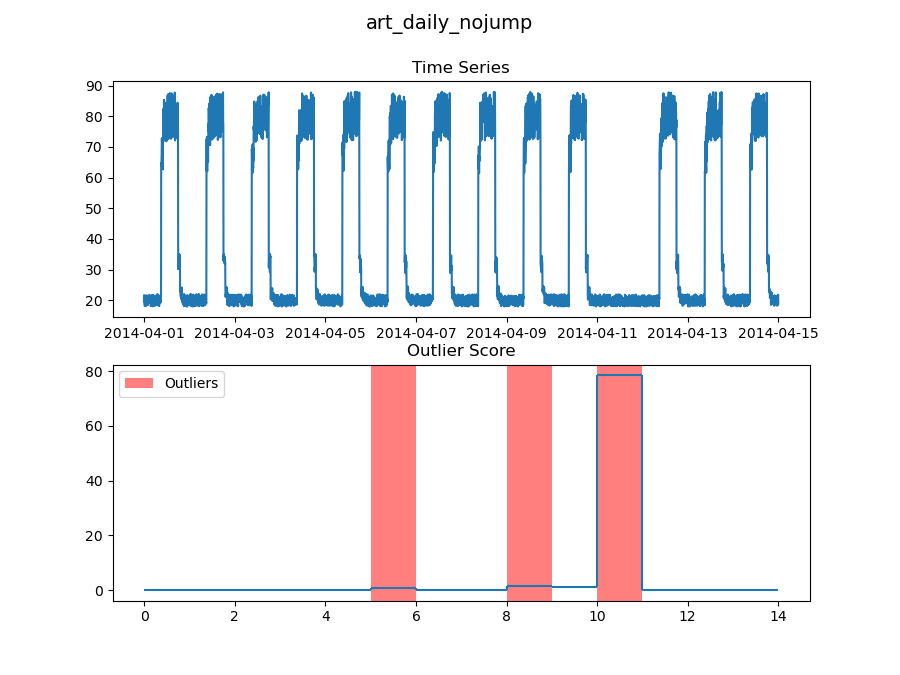
\includegraphics[width=0.5\textwidth]{fig/resultsNetismile/1D/art_daily_nojump}}
	\label{img:isomappictures2}
\end{figure}

\workTodo{Wrong picture for daily peaks. Change that the sixed element is not always an outlier}

\newpage
\section{Zweidimensionales Signal Optimierte Version}
\label{sec:appendix_net_two}
\begin{figure}
	\centering
	\subfloat[Caption for sub-figure1]{
		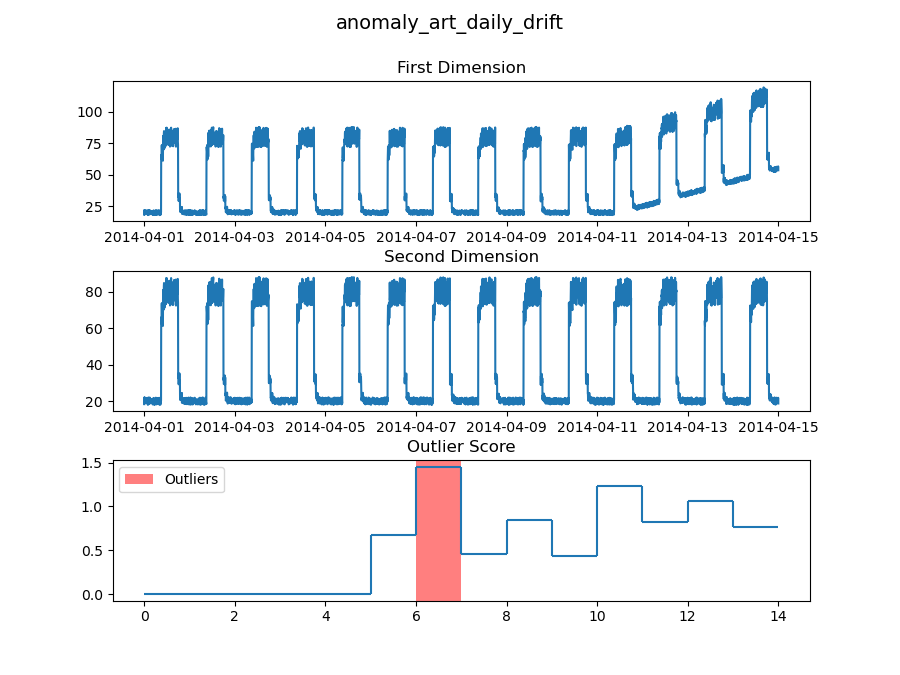
\includegraphics[width=0.5\textwidth]{fig/resultsNetismile/2D/anomaly_art_daily_drift}}
	\subfloat[Caption for sub-figure1]{
		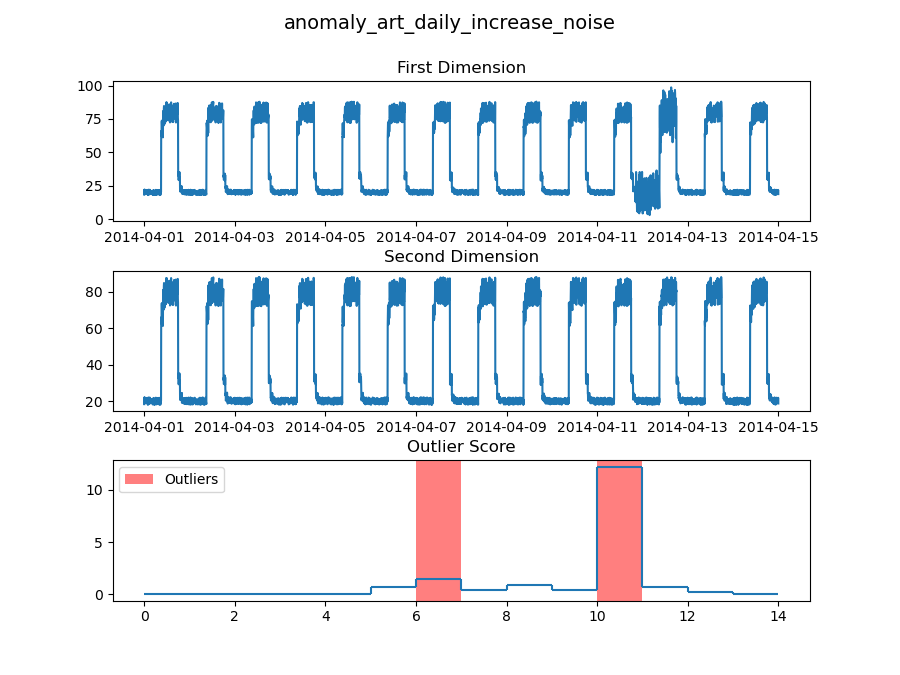
\includegraphics[width=0.5\textwidth]{fig/resultsNetismile/2D/anomaly_art_daily_increase_noise}}
	\qquad
	\subfloat[Caption for sub-figure1]{
		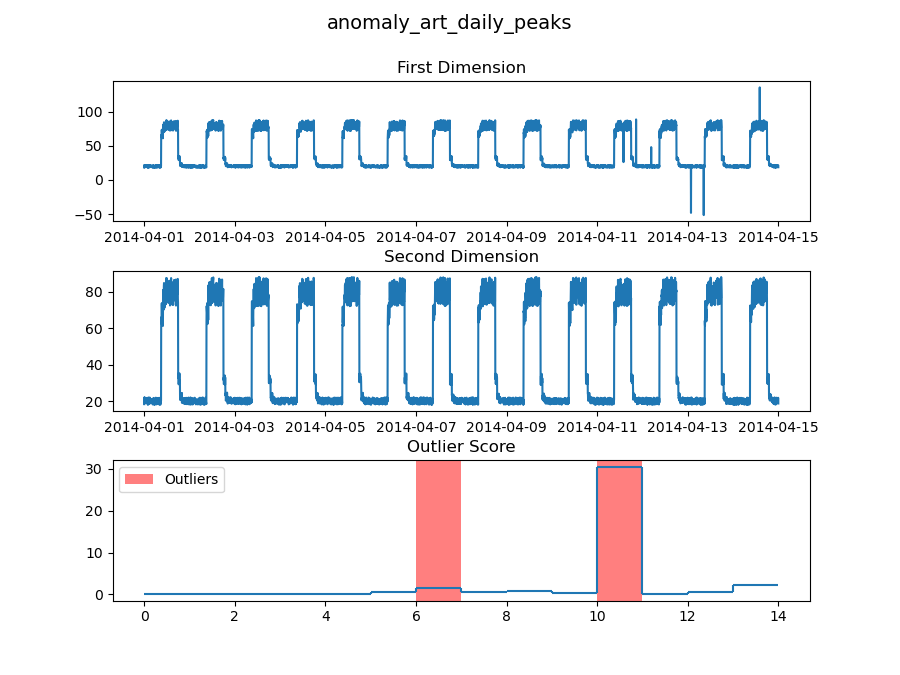
\includegraphics[width=0.5\textwidth]{fig/resultsNetismile/2D/anomaly_art_daily_peaks}}
	\subfloat[Caption for sub-figure1]{
		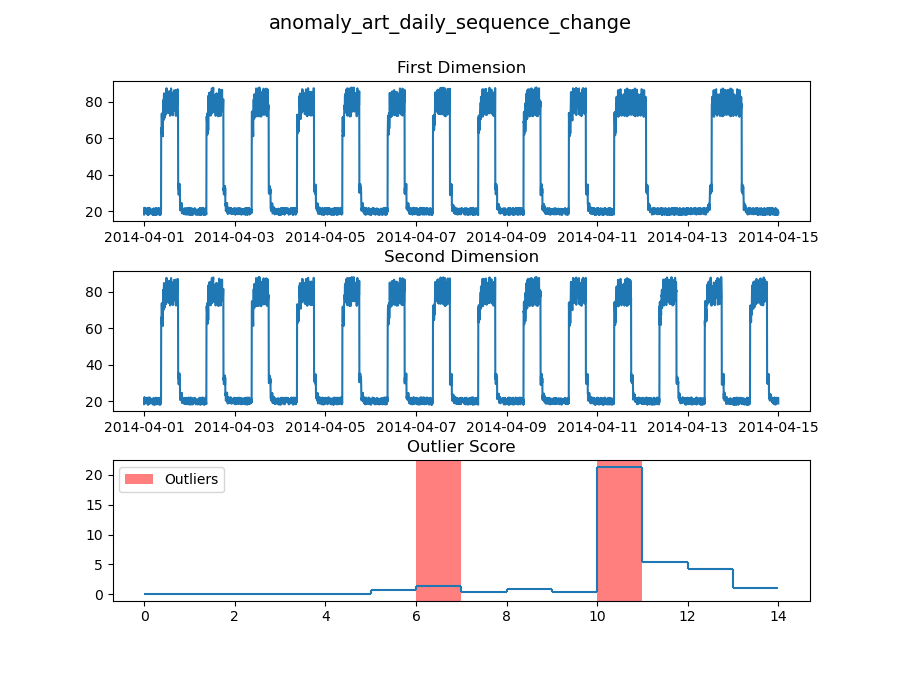
\includegraphics[width=0.5\textwidth]{fig/resultsNetismile/2D/anomaly_art_daily_sequence_change}}
	\qquad
	\label{img:isomappictures1}
\end{figure}
\begin{figure}\ContinuedFloat
	\subfloat[Caption for sub-figure1]{
		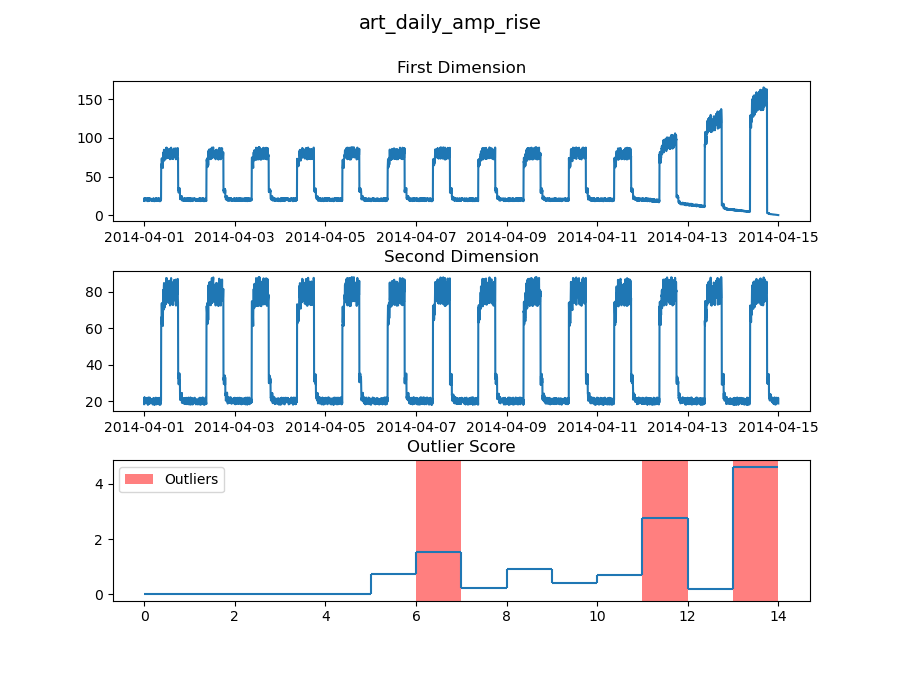
\includegraphics[width=0.5\textwidth]{fig/resultsNetismile/2D/art_daily_amp_rise}}
	\subfloat[Caption for sub-figure1]{
		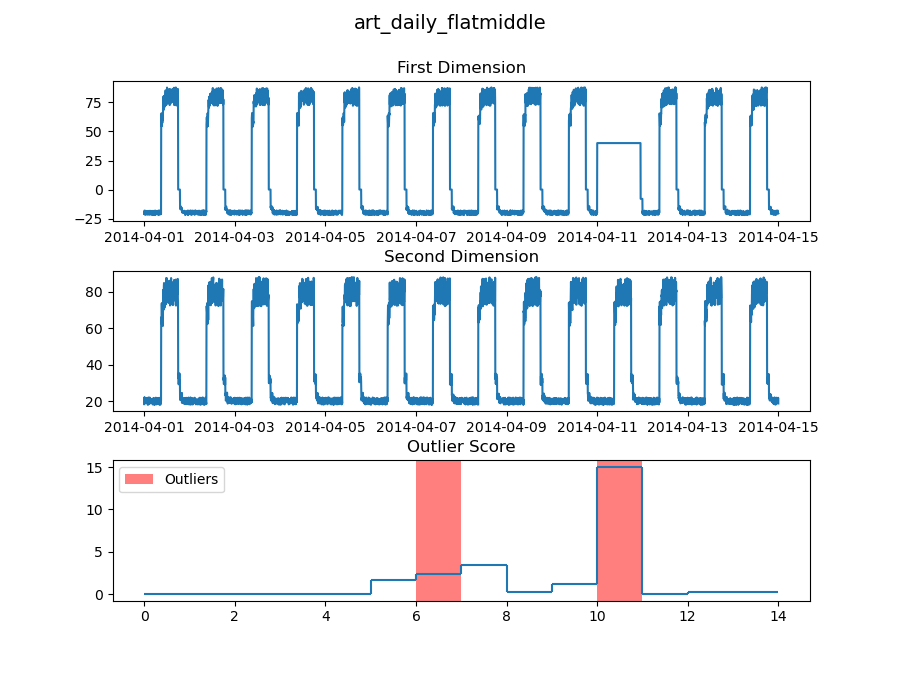
\includegraphics[width=0.5\textwidth]{fig/resultsNetismile/2D/art_daily_flatmiddle}}
	\qquad
	\subfloat[Caption for sub-figure1]{
		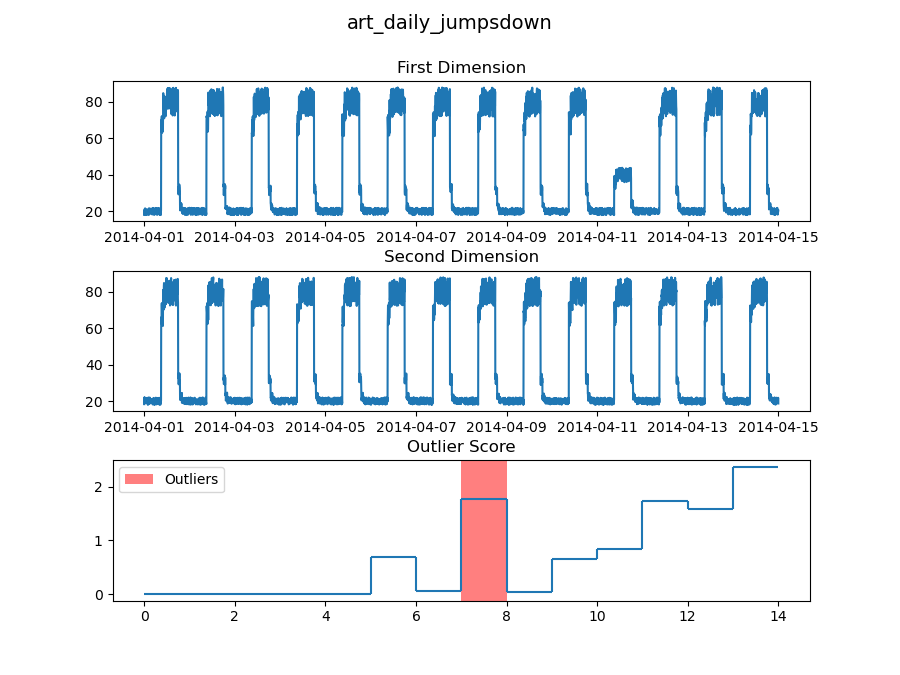
\includegraphics[width=0.5\textwidth]{fig/resultsNetismile/2D/art_daily_jumpsdown}}
	\subfloat[Caption for sub-figure1]{
		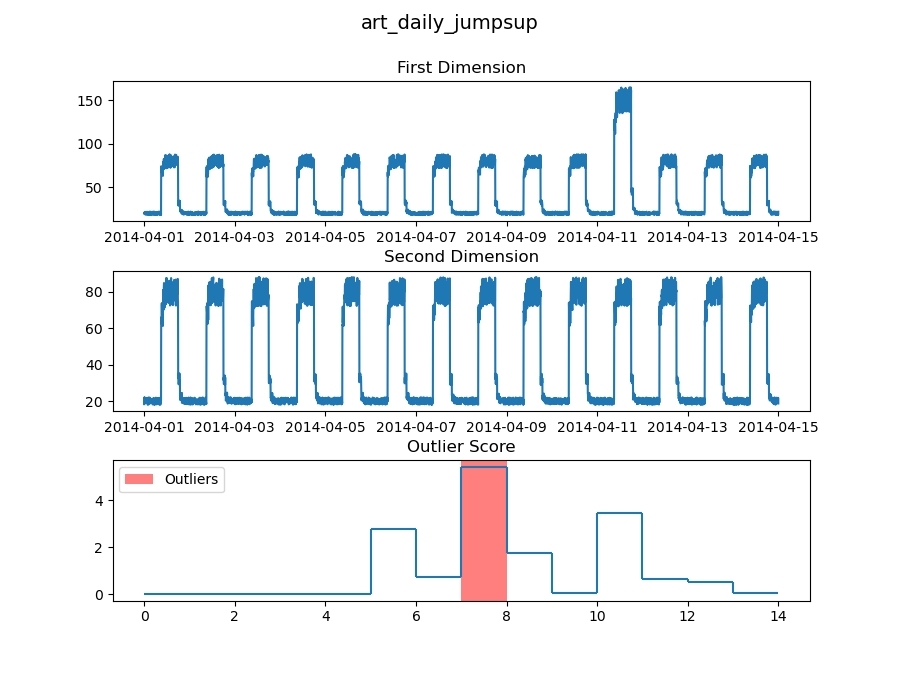
\includegraphics[width=0.5\textwidth]{fig/resultsNetismile/2D/art_daily_jumpsup}}
	\qquad
	\subfloat[Caption for sub-figure1]{
		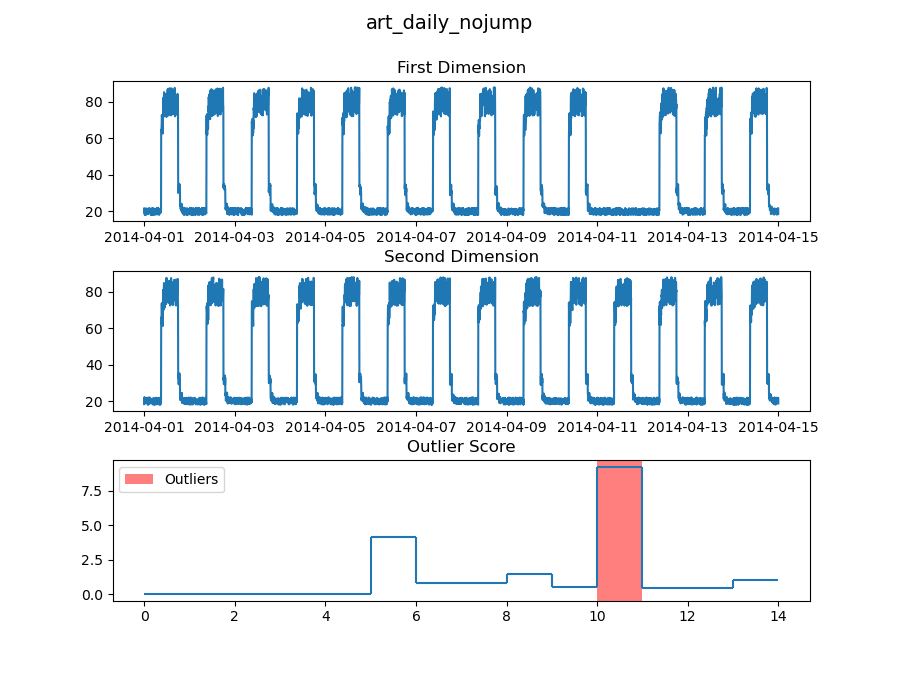
\includegraphics[width=0.5\textwidth]{fig/resultsNetismile/2D/art_daily_nojump}}
	\label{img:isomappictures2}
\end{figure}


\workTodo{Wrong picture for daily peaks. Change that the sixed element is not always an outlier}